\documentclass[12pt,a4paper]{article}
\usepackage[latin1]{inputenc}
\usepackage{amsmath}
\usepackage{amsfonts}
\usepackage{amsthm}
\usepackage{amssymb}
 \usepackage{stmaryrd}
\usepackage{fullpage}
\usepackage{listings}
 \usepackage{array}
\usepackage{hyperref}
\usepackage{setspace}
\usepackage[pdftex]{graphicx}
\usepackage{fixltx2e}
\newcommand{\mc}{\mathcal}
\newcommand{\dgmtversion}{1.2.0.4}
\newcommand{\HRule}{\rule{\linewidth}{0.5mm}}
\begin{document}

\begin{titlepage}

\begin{center}
\vspace*{\fill}

\begin{doublespace}
\textsc{\LARGE Parisian Master of Research in Computer Science}\\[1.5cm]
\end{doublespace}

\textsc{\Large Network programming project}\\[0.5cm]


% Title
\HRule \\[0.4cm]
{ \huge \bfseries MindTris Protocol Specification }\\[0.4cm]
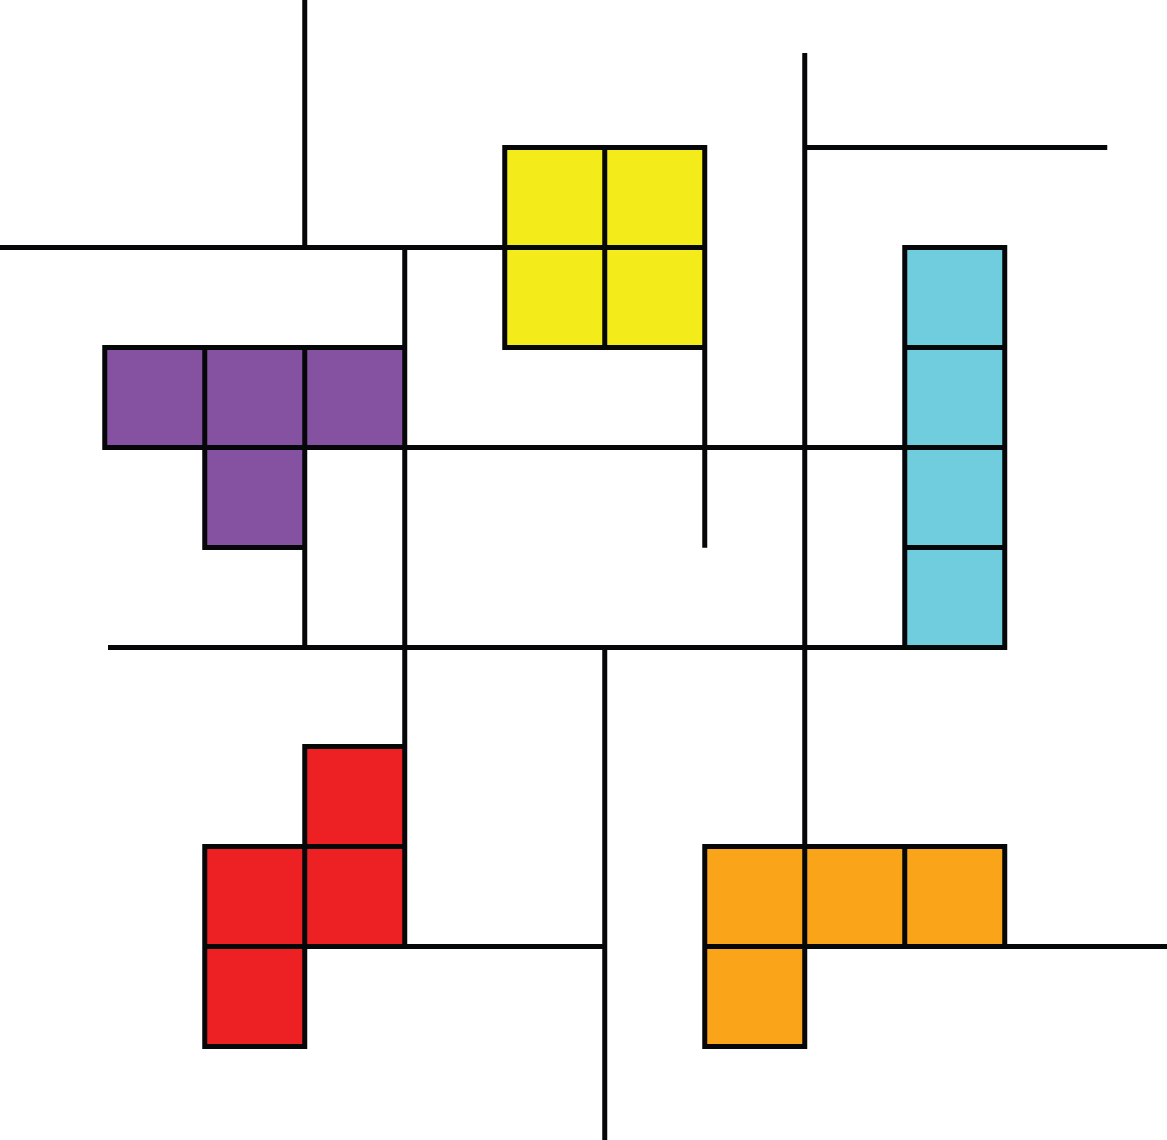
\includegraphics[width=0.15\textwidth]{mindtris_logo.pdf}\\[1cm]
{ \LARGE \bfseries DGMT Protocol }\\[0.4cm]
{\Large \bfseries Revision \dgmtversion  }
\HRule \\[1.5cm]

% Author and supervisor
\begin{minipage}{0.4\textwidth}
\begin{flushleft} \large
\emph{Authors:}\\
Charles-Pierre \textsc{Astolfi} \\
Rapha�l \textsc{Bonaque} \\
David \textsc{Montoya} \\
�mile \textsc{Contal} \\ 
Martin \textsc{Gleize}
\end{flushleft}
\end{minipage}
\begin{minipage}{0.4\textwidth}
\begin{flushright} \large
\emph{Supervisors:} \\
Thomas \textsc{Chatain} \\
Hedi \textsc{Benzina}
\end{flushright}
\end{minipage}

\vfill

{\large \today}

\end{center}

\end{titlepage}

\lstset{language=C++,basicstyle=\footnotesize}

\section{Naming conventions}

In this paper, packet structures for the DGMT protocol will be described in detail. We will employ the following types of terms:

\begin{itemize}

\item $data\_type$: the following data types will be employed:
\begin{itemize}
\item $void$: a void pointer. It can have take only value, \verb NULL . This will be used to refer to non assigned variables.
\item $byte$: an ordered collection of 8 bits. 
\item $int$: an integer of unspecified precision. We will employ both the decimal \verb [0-9]+  and hexadecimal \verb 0x[0-9A-F]+  notations in this paper. \\ \textbf{Implentors's note}: implementors are free to choose how they store integer data, as long as the precision employed is enough to represent the whole set of expectable values.
\item $int8$, $int16$, $int32$, $int64$: integers whose range is in comprised in $\llbracket 0, 2^x -1 \rrbracket $, where $x$ is equal to the number that appears in the name. 
\item $bool$: a boolean, whose value can be either $1$ or $0$.
\item $ustring$: a finite sequence of characters from the Unicode character set.
\item $data\_type[]$: an array of the specified $data\_type$.
\end{itemize}  
\item DATA\_ENCODING: a byte encoding of a given $data\_type$.
\item \verb CONSTANT_VALUE : a constant byte value, used to distinguish different message types or answers.
\item \verb variable : a variable used to store sensitive protocol data.
\end{itemize}  

\subsection{Encodings}
We define the following data encodings:

\begin{itemize}
\item BYTE: data is taken as "is", a $byte$ array is formed.
\item INTEGER: a big-endian integer encoding of an $int$. The actual interpretation depends on the number of bytes employed.
\item BOOLEAN: an encoding for a $bool$. Any non zero value represents $1$, while a zero value stands for $0$. If more than 1 byte is used, a $bool$ array is formed.
\item STRING: a ASCII encoding for $ustring$, using an arbitrary number of bytes.
\item USTRING: a UTF-8 encoding for $ustring$, using an arbitrary number of bytes.
\item ARRAY: an encoding for an array of arbitrary data. Individual data has particular encoding, and this data is concatenated at the byte level to form an array. The size of an ARRAY usually refers to the number of elements present in it.
\end{itemize}
\textbf{Implementor's note}: STRING can actually be interpreted as a USTRING without any loss of data. The reason we define the former is so that we can specify the kind of information we expect to have, although this should be done at a higher level of abstraction.

\section{Overview}

The DGMT protocol defines how a MindTris client can communicate with a MindTris server.


\subsection{Client's state information}

Clients must maintain the following state information for each server it connects to. We will describe the state information by defining a series of variables. By default, variables can be of two $data\_type$, one of which must be $void$. \\

\textbf{Implementor's note}: This information does not specify the implementation one should use, it merely gives information relevant to the validity of the protocol. For this reason, some information, which could be important for providing good user experience, will not necessarily be described here.

\begin{itemize}
\item \verb server_pub_key  ($byte[]$): The server's public RSA key. Used by the client in communications where secret transmission of data is necessary. This variable should include the modulus and exponent integer values of the key. The default value is \verb NULL .
\end{itemize}
The client keeps track of the current status of the client/server connection. This could be whether the client has logged in, is in a game, etc. It should include information such as following:
\begin{itemize}
\item \verb connected  ($bool$): Whether or not the client has received a positive handshake answer from the server. Defaults as 0.
\item \verb logged_on  ($bool$): Whether or not the client has successfully authenticated itself as a certain user existing in the server's database. Defaults as 0.
\item \verb user  ($ustring$): The user the client has authenticated as. Defaults as \verb NULL .
\item \verb lobby_id   ($int32$): The ID of the lobby the user has joined. Defaults as \verb NULL . 
\item \verb peer_id  ($int8$): The peer ID for the lobby the user is in. Defaults as \verb NULL . 
\item \verb creator_lobby_id  ($int32$): The ID of the lobby the user has created, if it has created any lobby. Defaults as \verb NULL .
\item \verb session_id  ($int64$): the id of the session the server has generated for the current game. Defaults as \verb NULL .
\item \verb am_playing ($bool$): Whether or not the user is in a game. Defaults as 0.
\end{itemize}

Conversely, server must maintain state information from each client it's connected to. This should include \verb connected , \verb logged_on , \verb ser , \verb lobby_id , \verb peer_id , \verb creator_lobby_id  and\verb am_playing. Additionally, it will include the client's public key (\verb client_pub_key ), which will be used for communications between peers to authenticate their messages. This key defaults as \verb NULL .\\

The server should at all times maintain information about lobbies that have been created, which will include their lobby ID, session ID and password. It should also keep a database of all registered users.


\subsection{Public Key message structure}

In some parts of the protocol, public RSA keys are expected to be transmitted. The expected format for such transmission is the following:

\begin{center}
  \begin{tabular}{|p{2cm}|c|c|c|p{8cm}|}
    \hline
    Name & Encoding & Size (B) & Default& Comment \\  \hline \hline
    Modulus Size & INTEGER & 2 & N/A & The size of the Modulus field. \\ \hline
   	Modulus & INTEGER & varies & N/A & The modulus part of the public key. \\ \hline
   	Exponent Size & INTEGER & 1 & N/A & The size of the Exponent field. \\ \hline
  	Exponent & INTEGER & varies & N/A & The modulus part of the public key. \\ \hline
  \end{tabular}
\end{center}

We will refer to this as the DGMT RSA Public Key format. \\

In other parts, a public DSA key is expected. This is the expected format:

\begin{center}
  \begin{tabular}{|p{2cm}|c|c|c|p{8cm}|}
    \hline
    Name & Encoding & Size (B) & Default& Comment \\  \hline \hline
    DSA\textsubscript{p} Size & INTEGER & 2 & N/A & The size of the DSA\textsubscript{p} field. \\ \hline
   	DSA\textsubscript{p} & INTEGER & varies & N/A & The modulus part of the public key. \\ \hline
   	DSA\textsubscript{q} Size & INTEGER & 2 & N/A & The size of the DSA\textsubscript{q} field. \\ \hline
  	DSA\textsubscript{q} & INTEGER & varies & N/A & The modulus part of the public key. \\ \hline
    DSA\textsubscript{g} Size & INTEGER & 2 & N/A & The size of the DSA\textsubscript{g} field. \\ \hline
   	DSA\textsubscript{g} & INTEGER & varies & N/A & The modulus part of the public key. \\ \hline
   	DSA\textsubscript{y} Size & INTEGER & 2 & N/A & The size of the DSA\textsubscript{y} field. \\ \hline
  	DSA\textsubscript{y} & INTEGER & varies & N/A & The modulus part of the public key. \\ \hline
  \end{tabular}
\end{center}


\section{Client-Server messages}

All packets sent between the server and the client must be structured as follows:

\begin{center}
  \begin{tabular}{|p{2cm}|c|c|c|p{8cm}|}
    \hline
    Name & Encoding & Size (B) & Default & Comment \\  \hline \hline
    Protocol & STRING & 4 & "DGMT" & Default protocol identifier. \\ \hline
    Size & INTEGER & 2 & & The size of the message in bytes, including the header. \\ \hline
    Payload & BYTE & varies & & The content of this field will vary depending on the type of message.\\ \hline
  \end{tabular}
\end{center}

\subsection{Hello}

This message is the first message in the handshake between the server and the client. The client will first send a \verb HELLO_FROM_CLIENT  message to the server, who in turn should answer with a \verb HELLO_FROM_SERVER  message.\\

\noindent \textbf{Request:}

\begin{center}
  \begin{tabular}{|p{2cm}|c|c|c|p{8cm}|}
    \hline
    Name & Encoding & Size (B) & Default & Comment \\  \hline \hline
    Type & INTEGER & 1 & 0x00 & This identifies the message as \verb HELLO_FROM_CLIENT . \\ \hline
    Protocol Version & INTEGER & 4 & \dgmtversion & Protocol/Client version; the format is xx.xx.xx.xx. \\ \hline
  \end{tabular}
\end{center}

\noindent \textbf{Response:}

\begin{center}
  \begin{tabular}{|p{2cm}|c|c|c|p{8cm}|}
    \hline
    Name & Encoding & Size (B) & Default& Comment \\  \hline \hline
    Type & INTEGER & 1 & 0x80 & This identifies the message as \verb HELLO_FROM_SERVER . \\ \hline
    Server Answer & INTEGER & 1 & N/A & Server's response. Must be one of the following:
    0x00 (\verb SUCCESS ), 0x01 (\verb WRONG_PROTOCOL_VERSION ), 0x02 (\verb UNKNOWN_ERROR ). \\ \hline
    Server's Public Key & BYTE & varies & N/A & The server's public RSA key. Used for transmission of secret data from the client to the server. The expected format is the DGMT RSA Public Key format. \\ \hline
    Message Size & INTEGER & 2 & N/A & The size of the Message field (bytes) \\ \hline
	Message & USTRING & varies & N/A & A human readable message from the server to the client. This could be a welcome message, if the Server Answer was \verb SUCCESS , or a few details about the error that occurred.\\ \hline
  \end{tabular}
\end{center}

If the server answers \verb SUCCESS , the client will store the server's public key in its \verb server_pub_key  variable. Additionally the state variable \verb connected  is set to 1. Any other messages exchanged between the server and the client assume that \verb connected  is 1.

\subsection{Keep alive}

Clients regularly send a message with an empty Payload to the server from the moment they received a \verb HELLO_FROM_SERVER . They are expected to do so every 60 seconds, otherwise the server will drop the connection, and terminate any ongoing transactions with the client.

\subsection{User creation}

By this process, a client can create a user to be stored in the server's database. The client will first send a \verb CREATE_USER  message to the server, who in turn should answer with a \verb USER_CREATION  message. This message is only valid when the client \verb connected  variable is set to 1.\\

\noindent \textbf{Request:}

\begin{center}
  \begin{tabular}{|p{2cm}|c|c|c|p{8cm}|}
    \hline
    Name & Encoding & Size (B) & Default & Comment \\  \hline \hline
    Type & INTEGER & 1 & 0x01 & This identifies the message as \verb CREATE_USER . \\ \hline
    Username Size & INTEGER & 1 & N/A & The size of the Username field.\\ \hline
    Username & USTRING & varies & N/A & A name used to login.\\ \hline
    Display Name Size & INTEGER & 1 & N/A  & The size of the Display Name field.\\ \hline
    Display Name & USTRING & varies & N/A & A name that will be displayed to other users.\\ \hline
    Email Size & INTEGER & 2 & N/A & The size of the Email field. This value cannot be greater than 320.\\ \hline
    Email & STRING & varies & N/A & An email address, used to recover a lost password.\\ \hline
    Encrypted Password Size & INTEGER & 2 & N/A & The size of the Encrypted Password field. \\ \hline
    Encrypted Password & BYTE & varies & N/A & We will describe this content below. \\ \hline
  \end{tabular}
\end{center}

The Encrypted Password field should contain the following data, encrypted with the RSAES-OAEP (RSA Encryption Scheme - Optimal Asymmetric Encryption Padding) (SHA-1) scheme, using \verb server_pub_key .

\begin{center}
  \begin{tabular}{|p{2cm}|c|c|c|p{8cm}|}
    \hline
    Name & Encoding & Size (B) & Default & Comment \\  \hline \hline
    Password & STRING & varies & N/A & The password that will be used to login. \\ \hline
  \end{tabular}
\end{center}

Valid usernames must match \verb [:alpha:][:alnum:_.-]* , and valid password must match \begin{center} \verb ^.*(?=.{6,})(?=.*[:alnum:])(?=.*[:punct:]).*$ \end{center}

\noindent \textbf{Response:}

\begin{center}
  \begin{tabular}{|p{2cm}|c|c|c|p{8cm}|}
    \hline
    Name & Encoding & Size (B) & Default & Comment \\  \hline \hline
    Type & INTEGER & 1 & 0x81 & This identifies the message as \verb USER_CREATION . \\ \hline
    Answer & BYTE & 1 & N/A &    \begin{itemize}    	\item 0x00: the user has been created with success.
    	\item 0x01: this username already exists.
		\item 0x02: invalid username.
	    \item 0x03: invalid password.
	    \item 0x04: invalid email.
	\end{itemize}
    \\ \hline
  \end{tabular}
\end{center}


\subsection{Login}

By this process, a client can login as a user present in the server's database. The client will first send a \verb LOGIN  message to the server, who in turn should answer with a \verb LOGIN_REPLY  message. This message is only valid when the client \verb connected  variable is set to 1.\\

\noindent \textbf{Request:}

\begin{center}
  \begin{tabular}{|p{2cm}|c|c|c|p{8cm}|}
    \hline
    Name & Encoding & Size (B) & Default & Comment \\  \hline \hline
    Type & INTEGER & 1 & 0x02 & This identifies the message as \verb LOGIN . \\ \hline
    Username Size & INTEGER & 1 & N/A  & The size of the Username field.\\ \hline
    Username & USTRING & varies & N/A & A name used to login.\\ \hline
    Encrypted Password Size & INTEGER & 2 & N/A & The size of the Encrypted Password field. \\ \hline
    Encrypted Password & BYTE & varies & N/A & We will describe this content below. \\ \hline
  \end{tabular}
\end{center}

The Encrypted User Login Info field should contain the following data, encrypted with the RSAES-OAEP (SHA-1) scheme, using \verb server_pub_key .

\begin{center}
  \begin{tabular}{|p{2cm}|c|c|c|p{8cm}|}
    \hline
    Name & Encoding & Size (B) & Default & Comment \\  \hline \hline
    Password & STRING & varies & N/A & The password that will be used to login. \\ \hline
  \end{tabular}
\end{center}

\noindent \textbf{Response:}

\begin{center}
  \begin{tabular}{|p{2cm}|c|c|c|p{8cm}|}
    \hline
    Name & Encoding & Size (B) & Default & Comment \\  \hline \hline
    Type & INTEGER & 1 & 0x82 & This identifies the message as \verb LOGIN_REPLY . \\ \hline
    Answer & BYTE & 1 & N/A &    \begin{itemize}    	\item 0x00: login success.
        \item 0x01: username does not exist.
    	\item 0x02: bad username/password.
		\item 0x03: too many tries, try again later.
	    \item 0x04: login success, but another instance was disconnected elsewhere.
	\end{itemize} \\ \hline
	Answer Payload & BYTE & varies & N/A & The content of this field is determined by the Answer field. \\ \hline
  \end{tabular}
\end{center}

When Answer is equal to 0x00, the Answer Payload field will contain the data structure below. It should be empty otherwise.

\begin{center}
  \begin{tabular}{|p{2cm}|c|c|c|p{8cm}|}
    \hline
    Name & Encoding & Size (B) & Default & Comment \\  \hline \hline
    Display Name Size & INTEGER & 1 & N/A  & The size of the Display Name field.\\ \hline
    Display Name & USTRING & varies & N/A & The user's name that is displayed to others.\\ \hline
  \end{tabular}
\end{center}


Normally, the server will only give a success response if the username and password provided by the client match in the server's database.  The variable \verb logged_on  is set to 1 and \verb user  is set to the provided username on both the server and the client's side.


\subsection{Lobby Creation}

By this process, a user can create a lobby. This is only possible if \verb logged_on  is set to 1, \verb lobby_id  is set to \verb NULL  and \verb creator_lobby_id  is set to \verb NULL .\\

\noindent \textbf{Request:}

\begin{center}
  \begin{tabular}{|p{2cm}|c|c|c|p{8cm}|}
    \hline
    Name & Encoding & Size (B) & Default & Comment \\  \hline \hline
    Type & INTEGER & 1 & 0x03 & This identifies the message as \verb CREATE_LOBBY . \\ \hline
    Lobby Name Size& INTEGER & 1 & N/A & The size of the Lobby Name field. \\ \hline
    Lobby Name& USTRING & varies & N/A & The name of the lobby to be created. \\ \hline
    Player Allowed Count & INTEGER & 1 & N/A & The maximum number of players allowed. \\ \hline
    Has Password& BOOLEAN & 1 & 0 & Whether or not the lobby will require a password. \\ \hline
    Encrypted Lobby Password Size & INTEGER & 2 & N/A & The size of the Encrypted Lobby Password field or empty if the Has Password field is 0.\\ \hline
    Encrypted Lobby Password & BYTE & varies & N/A & This field is empty if the Has Password field is 0. \\ \hline
   	Port number & INTEGER & 2 & N/A & The client's TCP listen port number, used for communication between peers.\\ \hline
    Client's Public Key & BYTE & varies & N/A & The client's public key, used to sign peer-to-peer messages. The expected format is the DGMT Public Key format. \\ \hline
  \end{tabular}
\end{center}

The Encrypted Lobby Password field, if provided, should contain the following data, encrypted with the RSA-OAEP (SHA-1) scheme, using \verb server_pub_key .

\begin{center}
  \begin{tabular}{|p{2cm}|c|c|c|p{8cm}|}
    \hline
    Name & Encoding & Size (B) & Default & Comment \\  \hline \hline
    Password & STRING & varies & N/A & The password that will requested to join the lobby. \\ \hline
  \end{tabular}
\end{center}

Note that a valid password must match \begin{center} \verb ^.*(?=.{6,})(?=.*[:alnum:])(?=.*[:punct:]).*$ \end{center}

\noindent \textbf{Response:}

\begin{center}
  \begin{tabular}{|p{2cm}|c|c|c|p{8cm}|}
    \hline
    Name & Encoding & Size (B) & Default & Comment \\  \hline \hline
    Type & INTEGER & 1 & 0x83 & This identifies the message as \verb LOBBY_CREATION . \\ \hline
    Answer & BYTE & 1 & N/A &    \begin{itemize}    	\item 0x00: lobby created with success.
        \item 0x01: invalid password.
	    \item 0x02: you do not have enough rights create a lobby.
	    \item 0x03: invalid number of players.
	    \item 0xFF: unknown error.
	\end{itemize} \\ \hline
	Lobby Creation Payload & BYTE & varies & N/A & The value of this field depends on the Answer field. This is described below. \\ \hline
  \end{tabular}
\end{center}

When Answer is equal to 0x00, the following information is included in the Lobby Creation Payload field:

\begin{center}
  \begin{tabular}{|p{2cm}|c|c|c|p{8cm}|}
    \hline
    Name & Encoding & Size (B) & Default & Comment \\  \hline \hline
    Lobby ID & INTEGER & 4 & N/A &  An ID generated by the server for the lobby than has been created. This value should be generated so that all current available lobbies have unique IDs.\\ \hline
	Peer ID & INTEGER & 1 & N/A & The creator peer's unique ID for this lobby. Used to identify peers during the game.\\ \hline 
	Session ID & INTEGER & 8 & N/A & This lobby's session's ID. Used in peer-to-peer messages to prevent clients from reusing signed packets. This is different from lobby ID in the sense that a Session ID is required to be unpredictable, while lobby IDs can be generated for efficient retrieval of lobby lists. \\ \hline
  \end{tabular}
\end{center}

The field is empty otherwise.

\subsection{Lobby List Retrieval}

Users might want to know the list of available lobbies. This is only possible if \verb logged_on  is set to 1. \\

\noindent \textbf{Request:}

\begin{center}
  \begin{tabular}{|p{2cm}|c|c|c|p{8cm}|}
    \hline
    Name & Encoding & Size (B) & Default & Comment \\  \hline \hline
    Type & INTEGER & 1 & 0x04 & This identifies the message as \verb GET_LOBBY_LIST . \\ \hline
  \end{tabular}
\end{center}

\noindent \textbf{Response:}


\begin{center}
  \begin{tabular}{|p{2cm}|c|c|c|p{8cm}|}
    \hline
    Name & Encoding & Size (B) & Default & Comment \\  \hline \hline
    Type & INTEGER & 1 & 0x84 & This identifies the message as \verb LOBBY_LIST . \\ \hline
    Lobby List Size & INTEGER & 1 & N/A & The size of the Lobby List array (number of elements). \\ \hline
    Lobby List & ARRAY & varies & N/A & An array of Lobby data, described  below. \\ \hline
  \end{tabular}
\end{center}

The Lobby List contains an array with the following data structure:

\begin{center}
  \begin{tabular}{|p{2cm}|c|c|c|p{8cm}|}
    \hline
    Name & Encoding & Size (B) & Default & Comment \\  \hline \hline
    Lobby ID & INTEGER & 4 & N/A & The lobby ID. \\ \hline
    Lobby Name Size& INTEGER & 1 & N/A & The size of the Lobby Name field. \\ \hline
    Lobby Name& USTRING & varies & N/A & The name of the lobby to be created. \\ \hline
    Player Count & INTEGER & 1 & N/A & The number of players present in the lobby. \\ \hline
    Player Allowed Count & INTEGER & 1 & N/A & The maximum number of players allowed. \\ \hline
    Password Protected & BOOLEAN & 1 & 0 & Whether or not this lobby requires a password to join. \\ \hline   
    Creator Size & INTEGER & 1 & N/A & The size of the Creator field. \\ \hline   
    Creator & USTRING & varies & N/A & The display name of the creator of this lobby. \\ \hline   
  \end{tabular}
\end{center}

\subsection{Joining a lobby}

Users can decide to join a particular lobby. This is only possible if \verb logged_on  is set to 1 and if \verb lobby_id  is \verb NULL .\\

\noindent \textbf{Request:}

\begin{center}
  \begin{tabular}{|p{2cm}|c|c|c|p{8cm}|}
    \hline
    Name & Encoding & Size (B) & Default & Comment \\  \hline \hline
    Type & INTEGER & 1 & 0x05 & This identifies the message as \verb JOIN_LOBBY . \\ \hline
    Lobby ID & INTEGER & 4 & N/A  & The lobby ID. \\ \hline
    Password Size & INTEGER & 1 & N/A & The size of the Password field.\\ \hline
    Password & STRING & varies & N/A & The lobby's password. \\ \hline
    IP Address & INTEGER & 4 & N/A & The client's IPv4 address, as described  in \href{http://tools.ietf.org/html/rfc791}{RFC 791}. \\ \hline
	Port number & INTEGER & 2 & N/A & The client's TCP listen port number, used for communication between peers.\\ \hline
    Client's Public Key & BYTE & varies & N/A & The client's public key, used to sign peer-to-peer messages. The expected format is the DGMT DSA Public Key format. \\ \hline
  \end{tabular}
\end{center}

\noindent \textbf{Response:}

\begin{center}
  \begin{tabular}{|p{2cm}|c|c|c|p{8cm}|}
    \hline
    Name & Encoding & Size (B) & Default & Comment \\  \hline \hline
    Type & INTEGER & 1 & 0x85 & This identifies the message as \verb JOINED_LOBBY . \\ \hline
    Lobby ID & INTEGER & 4 & N/A  & The lobby ID. \\ \hline
    Answer & BYTE & 1 & N/A &    \begin{itemize}    	\item 0x00: joined lobby with success.
        \item 0x01: wrong password
	    \item 0x02: lobby is full
	    \item 0x03: unknown error
	\end{itemize}\\ \hline
	Answer Payload & BYTE & varies & N/A & The content of this field is determined by the Answer field. \\ \hline
  \end{tabular}
\end{center}

When Answer is equal to 0x00, the Answer Payload field will contain the data structure below. It should be empty otherwise.

\begin{center}
  \begin{tabular}{|p{2cm}|c|c|c|p{8cm}|}
    \hline
    Name & Encoding & Size (B) & Default & Comment \\  \hline \hline
    Lobby Name Size& INTEGER & 1 & N/A & The size of the Lobby Name field. \\ \hline
    Lobby Name& USTRING & varies & N/A & The name of the lobby to be created. \\ \hline
    Player Allowed Count & INTEGER & 1 & N/A & The maximum number of players allowed. \\ \hline 
    Creator Peer ID & INTEGER & 1 & N/A & The Peer ID of the creator of this lobby. \\ \hline   
    Peer ID & INTEGER & 1 & N/A & The joining peer's unique ID for this lobby. Used to identify peers during the game.\\ \hline 
	Session ID & INTEGER & 8 & N/A & This lobby's session's ID. Used in peer-to-peer messages to prevent clients from reusing signed packets. This is different from lobby ID in the sense that a Session ID is required to be unpredictable, while lobby IDs can be generated for efficient retrieval of lobby lists. \\ \hline
    Client List Size & INTEGER & 1 & N/A & The size of the Client List array (number of elements). \\ \hline
    Client List & ARRAY & varies & N/A & An array of clients currently present in the lobby, described below. \\ \hline
  \end{tabular}
\end{center}

The Client List array should implement the following data structure:

\begin{center}
  \begin{tabular}{|p{2cm}|c|c|c|p{8cm}|}
    \hline
    Name & Encoding & Size (B) & Default & Comment \\  \hline \hline
    Peer ID & INTEGER & 1 & N/A & The peer's unique ID for this lobby. Used to identify peers during the game.\\ \hline 
    Display Name Size & INTEGER & 1 & N/A  & The size of the Display Name field.\\ \hline
    Display Name & USTRING & varies & N/A & The name used by the client.\\ \hline
    IP Address & INTEGER & 4 & N/A & The client's IPv4 address, as described  in \href{http://tools.ietf.org/html/rfc791}{RFC 791}. \\ \hline
    Port number & INTEGER & 2 & N/A & The client's TCP listen port number, used for communication between peers.\\ \hline
    Client's Public Key & BYTE & varies & N/A & The client's public key, used to sign peer-to-peer messages. The expected format is the DGMT DSA Public Key format. \\ \hline
  \end{tabular}
\end{center}

Once the server responds, both ends set the \verb lobby_id  variable for this client to the value given by 


\subsection{Leaving a Lobby}

A user can decide to leave a lobby. In this case, it sends the following message to the server:

\begin{center}
  \begin{tabular}{|p{2cm}|c|c|c|p{8cm}|}
    \hline
    Name & Encoding & Size (B) & Default & Comment \\  \hline \hline
    Type & INTEGER & 1 & 0x06 & This identifies the message as \verb LEAVE_LOBBY . \\ \hline
  \end{tabular}
\end{center}

Note that this message will only be valid if \verb logged_on  is set to 1 and if \verb lobby_id  is different than \verb NULL . The server, instead of responding directly to this message, will respond with an \verb UPDATE_CLIENT_STATUS  message, which is described in section \ref{updatelobby}.

\subsection{Kicking a user}

The user who created the lobby can decide to kick another user. This message has to be sent:

\begin{center}
  \begin{tabular}{|p{2cm}|c|c|c|p{8cm}|}
    \hline
    Name & Encoding & Size (B) & Default & Comment \\  \hline \hline
    Type & INTEGER & 1 & 0x07 & This identifies the message as \verb KICK_USER_FROM_LOBBY . \\ \hline
    Peer ID & INTEGER & 1 & N/A & The ID of the peer who will be kicked.\\ \hline 
  \end{tabular}
\end{center}

Note that this message will only be valid if \verb logged_on  is set to 1, \verb lobby_id  is different than \verb NULL  and if \verb creator  is set to 1. The server, instead of responding directly to this message, will respond with an \verb UPDATE_CLIENT_STATUS  message, which is described in section \ref{updatelobby}.


\subsection{Update client lobby status}
\label{updatelobby}
The server is supposed to notify clients in a lobby of any status updates from other clients joining, leaving or being kicked from the lobby. The server sends this message to all present clients (that is, those whose \verb lobby_id  matches the lobby in question), including the one whose status has been updated, if they happen to have been kicked or left the lobby.

\begin{center}
  \begin{tabular}{|p{2cm}|c|c|c|p{8cm}|}
    \hline
    Name & Encoding & Size (B) & Default & Comment \\  \hline \hline
    Type & INTEGER & 1 & 0x88 & This identifies the message as \verb UPDATE_CLIENT_STATUS. \\ \hline
    Lobby ID & INTEGER & 4 & N/A  & The ID of the lobby in question. \\ \hline
    Status Update & BYTE & 1 & N/A &    \begin{itemize}    	\item 0x00: has joined the lobby
        \item 0x01: has left the lobby
	    \item 0x02: has been kicked from the lobby
	\end{itemize}\\ \hline
    Peer ID & INTEGER & 1 & N/A & The ID of the peer whose status has been updated.\\ \hline 
    Status Payload & BYTE & varies & N/A & Depending on the type of Status Update, the content of this field will differ. \\ \hline
  \end{tabular}
\end{center}

When Status Update is equal to 0x00, the following information is included in the Status Payload field:

\begin{center}
  \begin{tabular}{|p{2cm}|c|c|c|p{8cm}|}
    \hline
    Name & Encoding & Size (B) & Default & Comment \\  \hline \hline
    Display Name Size & INTEGER & 1 & N/A  & The size of the Display Name field.\\ \hline
    Display Name & USTRING & varies & N/A & The name used by the joining client.\\ \hline
    IP Address & INTEGER & 4 &  N/A & The joining client's IPv4 address, as described  in \href{http://tools.ietf.org/html/rfc791}{RFC 791}. \\ \hline
    Port number & INTEGER & 2 & N/A & The joining client's TCP listen port number, used for communication between peers.\\ \hline
    Client's Public Key & BYTE & varies & N/A & The client's public key, used to sign peer-to-peer messages. The expected format is the DGMT DSA Public Key format. \\ \hline
  \end{tabular}
\end{center}

When the Status Update is equal to 0x01 or 0x02, clients are expected to terminate the connection they have with the corresponding peer. Additionally, the variable \verb lobby_id  is set to \verb NULL  and \verb creator  is set to 0.

\subsection{Starting a game}

Users having created a lobby can choose to start a game. They are easily identified for having \verb creator_lobby_id  different than \verb NULL .\\

\noindent \textbf{Request:}

\begin{center}
  \begin{tabular}{|p{2cm}|c|c|c|p{8cm}|}
    \hline
    Name & Encoding & Size (B) & Default & Comment \\  \hline \hline
    Type & INTEGER & 1 & 0x10 & This identifies the message as \verb START_GAME . \\ \hline
  \end{tabular}
\end{center}

\noindent \textbf{Response:}

\begin{center}
  \begin{tabular}{|p{2cm}|c|c|c|p{8cm}|}
    \hline
    Name & Encoding & Size (B) & Default & Comment \\  \hline \hline
    Type & INTEGER & 1 & 0x90 & This identifies the message as \verb GAME_STARTING. \\ \hline
    Answer & BYTE & 1 & N/A &    \begin{itemize}    	
    	\item 0x00: engaging with game start procedures.
	\end{itemize} \\ \hline 
  \end{tabular}
\end{center}

The server's answer is only interesting when an unknown error is triggered. Otherwise, a correct game start procedure will force the server into telling every client in the lobby matching the client's \verb creator_lobby_id  to start loading a game, a message we will describe in the next section.

\subsection{Loading a game}

The server can request clients having joined a certain lobby to start loading a game. Games can take a certain amount of time to allocate resources in a given client, which is why we expect clients to take some time before they give an answer to the server. Additionally, server includes first pieces to be played during the game.

\noindent \textbf{Request:}

\begin{center}
  \begin{tabular}{|p{2cm}|c|c|c|p{8cm}|}
    \hline
    Name & Encoding & Size (B) & Default & Comment \\  \hline \hline
    Type & INTEGER & 1 & 0x91 & This identifies the message as \verb LOAD_GAME . \\ \hline
    First Pieces Array Size & INTEGER & 1 & 10 & The size of the First Pieces array. \\ \hline
    First Pieces & ARRAY & varies & N/A & An array including the IDs of the first pieces being played, each of them is encoded as 1-byte INTEGER. \\ \hline
  \end{tabular}
\end{center}

Note: Pieces are encoded from 0 to 6, as follows:

\begin{center}
  \begin{tabular}{|c|c|}
    \hline
 	Piece Name &   Piece ID\\  \hline \hline
	I & 0 \\ \hline
	J & 1 \\ \hline
	L & 2 \\ \hline
	O & 3 \\ \hline
	S & 4 \\ \hline
	T & 5 \\ \hline
	Z & 6 \\ \hline
  \end{tabular}
\end{center}

\noindent \textbf{Response:}

\begin{center}
  \begin{tabular}{|p{2cm}|c|c|c|p{8cm}|}
    \hline
    Name & Encoding & Size (B) & Default & Comment \\  \hline \hline
    Type & INTEGER & 1 & 0x11 & This identifies the message as \verb LOADED_GAME. \\ \hline
    Answer & BYTE & 1 & N/A &    
    \begin{itemize}    	
		\item 0x00: loaded game, connected to all peers
		\item 0x01: can't connect to certain peers
	\end{itemize}\\ \hline 
	Answer Payload & BYTE & varies & N/A & The content of this field is determined by the Answer field. \\ \hline
  \end{tabular}
\end{center}

When Answer is equal to 0x01, the Answer Payload field will contain the data structure below. It should be empty otherwise.

\begin{center}
  \begin{tabular}{|p{2cm}|c|c|c|p{8cm}|}
    \hline
    Name & Encoding & Size (B) & Default & Comment \\  \hline \hline
	Peer ID Array Size & INTEGER & 1 & N/A & The size of the peer ID array. \\ \hline 
	Peer IDs& ARRAY & varies & N/A & The IDs of each of peer this peer couldn't connect to. Each of these is represented as a 1-byte INTEGER. \\ \hline 
  \end{tabular}
\end{center}

\subsection{Beginning of a game}

The server, once it received a successful \verb LOADED_GAME  answer from all connected players, will decide as to the beginning of a game. It will simply send this message to all of them:

\begin{center}
  \begin{tabular}{|p{2cm}|c|c|c|p{8cm}|}
    \hline
    Name & Encoding & Size (B) & Default & Comment \\  \hline \hline
    Type & INTEGER & 1 & 0x92 & This identifies the message as \verb BEGIN_GAME . \\ \hline
  \end{tabular}
\end{center}


\subsection{Obtaining new pieces}

The server is responsible for telling each player about the next pieces to be played. It can do so any time it wishes. For this purpose, this message is sent to each client:

\begin{center}
  \begin{tabular}{|p{2cm}|c|c|c|p{8cm}|}
    \hline
    Name & Encoding & Size (B) & Default & Comment \\  \hline \hline
    Type & INTEGER & 1 & 0x93 & This identifies the message as \verb NEW_PIECES . \\ \hline
    Piece Number Offset & INTEGER & 4 & N/A & The number of the first piece in the Pieces array.\\ \hline
    Pieces Array Size & INTEGER & 1 & 10 & The size of the Pieces array. \\ \hline
    Pieces & ARRAY & varies & N/A & An array including the IDs of the new pieces, each of them is encoded as 1-byte INTEGER. \\ \hline
  \end{tabular}
\end{center}

Additionally, clients can encourage the server to do so:

\begin{center}
  \begin{tabular}{|p{2cm}|c|c|c|p{8cm}|}
    \hline
    Name & Encoding & Size (B) & Default & Comment \\  \hline \hline
    Type & INTEGER & 1 & 0x13 & This identifies the message as \verb GIVE_NEW_PIECES . \\ \hline
    Piece Number Offset & INTEGER & 4 & N/A & The number of the first piece requested.\\ \hline
    Piece Requested Number & INTEGER & 1 & N/A & The number of pieces requested.\\ \hline
  \end{tabular}
\end{center}

Reaction by the server to this message is done at the server's discretion.

\subsection{End of a game}

Clients send the results of a game to the server when it finishes:

\begin{center}
  \begin{tabular}{|p{2cm}|c|c|c|p{8cm}|}
    \hline
    Name & Encoding & Size (B) & Default & Comment \\  \hline \hline
    Type & INTEGER & 1 & 0x14 & This identifies the message as \verb GAME_END . \\ \hline
	Results Array Size & INTEGER & 1 & N/A & The size of the Results array. \\ \hline
	Results & ARRAY & varies & N/A & An array of results for each different client. \\ \hline
  \end{tabular}
\end{center}

The Results array will include the following:

\begin{center}
  \begin{tabular}{|p{2cm}|c|c|c|p{8cm}|}
    \hline
    Name & Encoding & Size (B) & Default & Comment \\  \hline \hline
    Peer ID & INTEGER & 1 & N/A & The ID of the peer whose result is from.\\ \hline 
    Winning Rank & INTEGER & 1 & N/A & Ranks determine the order at which players lost. The player who ultimately won should be rank 1. Players whose rank can't be determined should be rank 0.\\ \hline
    Score & INTEGER & 4 & N/A & The score of the client at the end of the game. \\ \hline
  \end{tabular}
\end{center}


\section{Peer-to-Peer messages}
 
Peer-to-peer messages work inherently different from Server/Client messages. Unlike the former, peer-to-peer do not follow a request-response pattern. 
%The protocol is intended to be used with UDP, using UDP hole punching to traverse NATs. For this reason, most answer messages are expected to be acknowledgements.

All packets sent between the peers must be structured as follows:

\begin{center}
  \begin{tabular}{|p{2cm}|c|c|c|p{8cm}|}
    \hline
    Name & Encoding & Size (B) & Default & Comment \\  \hline \hline
    Protocol & STRING & 7 & "DGMTP2P" & Default protocol identifier. \\ \hline
    Size & INTEGER & 2 & & The size of the message in bytes, including the header. \\ \hline
    Payload & BYTE & varies & & The content of this field will vary depending on the type of message.\\ \hline
  \end{tabular}
\end{center}

Basically, clients are expected to connect to each other the moment they join a lobby. The client having joined last must initiate the connection. They must use the TCP port each individual peer is listening to, as provided by the server. Before they engage in any conversation, they must go through a handshake phase.

\subsection{Handshake}

Before engaging in any real communication, peers must authenticate with each other, by following a secure three-way handshake procedure.

During this phase, one peer initiates the connection. This is done by sending a \verb CONNECTION_REQUEST  message, to which the other peer will respond with a \verb CONNECTION_ACCEPTED  message, if the request is valid. The handshake ends with the peer's initiating sending a \verb CONNECTION_ACKNOWLEDGED  message, acknowledging the other peer's authenticity, and responding to the other's peer challenge.\\

\textbf{Connection request}

\begin{center}
  \begin{tabular}{|p{2cm}|c|c|c|p{8cm}|}
    \hline
    Name & Encoding & Size (B) & Default & Comment \\  \hline \hline
    Type & INTEGER & 1 & 0x00 & This identifies the message as \verb CONNECTION_REQUEST \\ \hline
    Lobby ID & INTEGER & 4 & N/A  & The lobby ID the peers are connected to. \\ \hline    
    Initiating Peer ID & INTEGER & 1 & N/A & The ID of the peer who initiates the connection.\\ \hline 
 	Listening Peer ID & INTEGER & 1 & N/A & The ID of the peer that accepts the connection. \\ \hline
    Initiating Challenge Code & INTEGER & 8 & N/A & A random number issued by the peer initiating the connection, for the purpose of only one handshake attempt.\\ \hline 
  \end{tabular}
\end{center}

The peer accepting the connection, will check whether the Lobby ID, Initiating Peer ID and Listening Peer ID are valid. If they are not, he should terminate the TCP connection. Otherwise he will send the following message: \\

\textbf{Connection challenge accepted}

\begin{center}
  \begin{tabular}{|p{2cm}|c|c|c|p{8cm}|}
    \hline
    Name & Encoding & Size (B) & Default & Comment \\  \hline \hline
    Type & INTEGER & 1 & 0x01 & This identifies the message as \verb CONNECTION_ACCEPTED \\ \hline
    Lobby ID & INTEGER & 4 & N/A  & The lobby ID the peers are connected to. \\ \hline    
    Initiating Peer ID & INTEGER & 1 & N/A & The ID of the peer who initiates the connection.\\ \hline 
 	Listening Peer ID & INTEGER & 1 & N/A & The ID of the peer that accepts the connection \\ \hline
    Initiating Challenge Code & INTEGER & 8 & N/A & The challenge code issued by the peer initiating the connection.\\ \hline 
    Listening Challenge Code & INTEGER & 8 & N/A & A random number issued by the peer accepting the connection, for the purpose of only one handshake attempt.\\ \hline 
    Signature Size & INTEGER & 2 & N/A & The size of the signature field in bytes. \\ \hline
    Signature & BYTE & varies & N/A & The accepting peer's signature for the message between the Lobby ID and Listening Challenge Code. The signature is generated by the Digital Signature Algorithm. \\ \hline
  \end{tabular}
\end{center}

The peer initiating the connection will check if the message corresponds to an ongoing handshake request, and verify that the signature matches the one it has for the peer accepting the connection, as provided by the server. If the message is not valid, he should terminate the TCP connection. Otherwise, the peer will assume that he has initiated a connection with the proper peer, and will send the final message: \\

\textbf{Connection Challenge Acknowledged}

\begin{center}
  \begin{tabular}{|p{2cm}|c|c|c|p{8cm}|}
    \hline
    Name & Encoding & Size (B) & Default & Comment \\  \hline \hline
    Type & INTEGER & 1 & 0x02 & This identifies the message as \verb CONNECTION_ACKNOWLEDGED \\ \hline
    Lobby ID & INTEGER & 4 & N/A  & The lobby ID the peers are connected to. \\ \hline    
    Initiating Peer ID & INTEGER & 1 & N/A & The ID of the peer who initiates the connection.\\ \hline 
 	Listening Peer ID & INTEGER & 1 & N/A & The ID of the peer that accepts the connection \\ \hline
    Initiating Challenge Code & INTEGER & 8 & N/A & The challenge code issue by the peer initiating the connection.\\ \hline 
    Listening Challenge Code & INTEGER & 8 & N/A & The challenge code issued by the peer accepting the connection.\\ \hline 
    Signature Size & INTEGER & 2 & N/A & The size of the signature field in bytes. \\ \hline
    Signature & BYTE & varies & N/A & The initiating peer's signature for the message between the Lobby ID and Listening Challenge Code. The signature is generated by the Digital Signature Algorithm. \\ \hline
  \end{tabular}
\end{center}

The accepting peer will verify that the fields match a previous \verb CONNECTION_ACCEPTED , and then check the signature for the peer initiating the connection, as provided by the server. If OK, he assumes that a connection has been established with the proper peer. Otherwise, he should terminate the TCP connection.

\subsection{Chat}

Chat messages don't rely on the server for transmission. They are sent directly to each peer.

\noindent \textbf{Chat Message:}

\begin{center}
  \begin{tabular}{|p{2cm}|c|c|c|p{8cm}|}
    \hline
    Name & Encoding & Size (B) & Default & Comment \\  \hline \hline
    Type & INTEGER & 1 & 0x10 & This identifies the message as \verb CHAT_SEND . \\ \hline
	Session ID & INTEGER & 8 & N/A & The lobby's session's ID. This makes reusing of old signed packets harder.\\ \hline
    Chat Message Length & INTEGER & 2 & N/A & The size of the Chat Message field. \\ \hline
    Chat Message & USTRING & varies & N/A & A chat message sent by the peer we are connected to. \\ \hline
    Signature Size & INTEGER & 2 & N/A & The size of the signature field in bytes. \\ \hline
    Signature & BYTE & varies & N/A & The client's RSA signature for the Session ID and Chat message, generated with DSA. \\ \hline
  \end{tabular}
\end{center}

\subsection{Game Round packets}

Most importantly, peers are supposed to send each other packets for each round that has been played. Rounds happen every 100ms.

\begin{center}
  \begin{tabular}{|p{2cm}|c|c|c|p{8cm}|}
    \hline
    Name & Encoding & Size (B) & Default & Comment \\  \hline \hline
    Type & INTEGER & 1 & 0x11 & This identifies the message as \verb ROUND . \\ \hline
    Round Data & BYTE & varies & N/A & The data about the round, this is described below. \\ \hline
    Signature Size & INTEGER & 2 & N/A & The size of the signature field in bytes. \\ \hline
    Signature & BYTE & varies & N/A & The client's RSA signature for the Round Data field, generated with DSA. \\ \hline
  \end{tabular}
\end{center}

Round Data include a bunch of gameplay dependent data.

\begin{center}
  \begin{tabular}{|p{2cm}|c|c|c|p{8cm}|}
    \hline
    Name & Encoding & Size (B) & Default & Comment \\  \hline \hline
	Session ID & INTEGER & 8 & N/A & The lobby's session's ID. This makes reusing of old signed packets harder.\\ \hline
	Round Number & INTEGER & 4 & N/A & The round number. Games start at round number 0, and this number increases by 1 for each subsequent round.\\ \hline
	Moves Array Size & INTEGER & 1 & N/A & The size of the Moves array.\\ \hline	
	Moves & ARRAY & varies & N/A & An array of moves the player has made during the round.\\ \hline	
    Round Data Hashes Array Size & INTEGER & 1 & N/A & The size of the Round Data Hashes field. \\ \hline
    Round Data Hashes & ARRAY & varies & N/A & An array of peer hashes, this is described next.\\ \hline
  \end{tabular}
\end{center}

The Tetris board is a rectangle of 10 columns by 20 rows. The X and Y offset range between 0-9, and 0-19, respectively. The location of a piece is given by the X and Y offset of the bottom left corner of the rectangle that perfectly bounds the piece, given its current orientation. The Moves array will include the following:

\begin{center}
  \begin{tabular}{|p{2cm}|c|c|c|p{8cm}|}
    \hline
    Name & Encoding & Size (B) & Default & Comment \\  \hline \hline
    Piece Number & INTEGER & 4 & N/A & The number of the piece being moved. Games start with piece number 0, and this number increases by 1 for each new piece that comes. \\ \hline
    Piece Orientation & INTEGER & 1 & N/A & The orientation of the piece. The default piece position is 0x00, and this number increases by 1 each time the piece is rotated in a clockwise fashion. \\ \hline
    Piece X Offset& INTEGER & 1 & N/A & The X offset of the location where the piece has been dropped.\\ \hline
    Piece Y Offset& INTEGER & 1 & N/A & The Y offset of the location where the piece has been dropped.\\ \hline
  \end{tabular}
\end{center}

The Round Data Hashes array should include the following information for each player present in the game.

\begin{center}
  \begin{tabular}{|p{2cm}|c|c|c|p{8cm}|}
    \hline
    Name & Encoding & Size (B) & Default & Comment \\  \hline \hline
    Peer ID & INTEGER & 1 & N/A & The Peer ID of the peer whose hash is from.\\ \hline 
    Round Data Hash & BYTE & 20 & N/A & The SHA-1 hash of the Round Data field sent by the above client.\\ \hline
  \end{tabular}
\end{center}

\subsection{Keep alive}

Peers regularly send each other a message with an empty Payload to the server from the moment they established a connection. They are expected to do so every 60 seconds.

\subsection{Relaying}

It is possible for peers connected to the same lobby to relay messages between each other. This can be useful when the peer-to-peer network is a ring or a tree. For this purpose, they use the following message structure:


\noindent \textbf{From Message:}

\begin{center}
  \begin{tabular}{|p{2cm}|c|c|c|p{8cm}|}
    \hline
    Name & Encoding & Size (B) & Default & Comment \\  \hline \hline
    Type & INTEGER & 1 & 0x12 & This identifies the message as \verb MESSAGE_FROM . \\ \hline
    From Peer ID & INTEGER & 1 & N/A & The ID of the peer whose the message comes from. \\ \hline 
    Message Length & INTEGER & 2 & N/A & The size of the Message field. \\ \hline
    Message & BYTE & varies & N/A & A DGMTP2P message, which includes the header. \\ \hline
  \end{tabular}
\end{center}

\end{document}